\documentclass{ctexart}

\usepackage[nea]{van-de-la-sehen}
\DeclareMathOperator{\sinc}{sinc}

\begin{document}

\section{光的干涉} % (fold)
\label{sec:光的干涉}

\subsection{分波前干涉装置} % (fold)
\label{sub:分波前干涉装置}

\subsubsection{各种分波前干涉装置} % (fold)
\label{ssub:各种分波前干涉装置}

\begin{figure}[hb]
    \centering
    \incfig{12cm}{SplitWavefront}
    \caption{分波前干涉装置}
\end{figure}
两束光在交叠区域里任意点$P$激起振动的初相位为
\[ \begin{aligned}
    \varphi_1\pare{P} &= \varphi_0 + \frac{2\pi}{\lambda} \pare{S\mathrm{I}P},\\
    \varphi_2\pare{P} &= \varphi_0 + \frac{2\pi}{\lambda} \pare{S\mathrm{II}P}.
\end{aligned} \]
Young干涉装置的公式可径直迁移至此类型的干涉装置.

\paragraph{Fresnel双面镜} % (fold)
\label{par:fresnel双面镜}

\begin{figure}[ht]
    \centering
    \incfig{12cm}{FresnelMirror}
    \caption{Fresnel双面镜}
\end{figure}
\begin{figure}[ht]
    \centering
    \incfig{12cm}{FresnelPrism}
    \caption{Fresnel双棱镜}
\end{figure}
$S$对$OO_1$成像于$S_1$, 对$OO_2$成像于$S_2$, 则
\[ \angle S_1OS_2 = 2\alpha\Rightarrow \Delta x = \frac{B+C}{2\alpha B}\lambda. \]

% paragraph fresnel双面镜 (end)

\paragraph{Fresnel双棱镜} % (fold)
\label{par:fresnel双棱镜}

\begin{figure}[ht]
    \centering
    \begin{subfigure}{.47\textwidth}
        \centering
        \incfig{5cm}{FirstRayFresnelPrism}
        \caption{Fresnel双棱镜平行出射}
        \label{fig:Fresnel双棱镜平行出射}
    \end{subfigure}
    \begin{subfigure}{.47\textwidth}
        \centering
        \incfig{5cm}{SecondRayFresnelPrism}
        \caption{Fresnel双棱镜平行入射}
        \label{fig:Fresnel双棱镜平行入射}
    \end{subfigure}
    \caption{Fresnel双棱镜二特殊光线}
\end{figure}
\begin{figure}[ht]
    \centering
    \incfig{12cm}{LloydMirror}
    \caption{Lloyd镜}
\end{figure}
\begin{figure}
    \centering
    \incfig{10cm}{DisplacementOfInterferograms}
    \caption{干涉条纹的位移}
\end{figure}

考虑两条特殊光线. 如\cref{fig:Fresnel双棱镜平行出射}, 第一条是出射水平者. 由折射定律,
\[ \begin{cases}
    1\cdot \sin i = n\sin r,\\
    n\sin r' = 1\cdot \sin i'.
\end{cases} \]
由$i' =\alpha$, $\alpha = r+r'$,
\begin{align*}
    \sin i &= n\sin r = n\sin\pare{\alpha - r'} = n\pare{\sin\alpha\cos r' - \cos\alpha\sin r'}. \\
    n\sin r' &= \sin \alpha. \\
    n\cos r' &= n\sqrt{1-\sin^2 r'} = \sqrt{n^2 - \sin^2 r}, \\
    \sin i &= \sin \alpha \brac{\sqrt{n^2 - \sin^2\alpha}} - \cos\alpha.
\end{align*}
如\cref{fig:Fresnel双棱镜平行入射}, 对于第二条光线, 在正入射的情形下(见第一章习题)
\begin{align*}
    n\sin \alpha& = 1\cdot \sin i'_0\Rightarrow i'_0 = n\cdot\alpha,\quad \beta = i'_0 - \alpha = \pare{n-1}\alpha. \\
    i &= \beta = \pare{n-1}\alpha. \\
    \frac{d}{2} &= B\alpha \pare{n-1}. \\
    \Delta x &= \frac{D}{d}\lambda = \frac{B+C}{2\pare{n-1}\alpha B}\lambda.
\end{align*}

% paragraph fresnel双棱镜 (end)

\paragraph{Lloyd镜} % (fold)
\label{par:lloyd镜}

\[ \Delta x = \frac{D}{2a}\lambda. \]
当接收光屏接触$N$, 结果为暗条纹而非根据表观光程计算所得相长干涉. 这是因为$n_1<n_2$时, 掠入射发生半波损失.

% paragraph lloyd镜 (end)

\paragraph{干涉条纹的移动} % (fold)
\label{par:干涉条纹的移动}

当光程差发生改变$\Delta L = j\lambda$, 则移动过$P$点的条纹数目$N$满足$\delta \pare{\Delta L} = N\lambda$. $\Delta x' = D\lambda / d$, 从而
\[ \delta x' = \frac{D}{d} N\lambda,\quad \delta x = \frac{R}{d}N\lambda. \]
中心条纹移动距离
\[ \delta x' = \frac{D}{R}\delta x. \]
\begin{remark}
    条纹的移动方向抵消光源移动导致的光程该变量. 例如$S$向下移动, 上方光线的光程变大, 故条纹向上移动以抵消其影响.
\end{remark}
\begin{remark}
    如果$S$朝纸面外侧移动, 则条纹不动, 因为不引入光程差改变.
\end{remark}

% paragraph 干涉条纹的移动 (end)

\paragraph{光源宽度对条纹反衬度的影响} % (fold)
\label{par:光源宽度对条纹反衬度的影响}

$y$方向的宽度对干涉时有利的, 惟$x$方向的宽度将会影响干涉条纹.
\begin{align*}
    I\pare{x',y'} &= I_0\pare{1+\cos \frac{kdx'}{D}}. \\
    I\pare{x'} &= I_0 \int_{-b/2}^{b/2} \brac{1+\cos \frac{kd}{D}\pare{x' - \frac{D}{R}x}}\,\rd{x} \\
    &= I_0 b \brac{1+\frac{\sin}{u}\cos \frac{kdx'}{D}}. \\
    \delta x' &= \frac{D}{R}\delta x,\quad u = \frac{kd}{R}\cdot \frac{b}{2}. \\
    I_{\mathrm{max}} &= I_0 b \brac{1+\abs{\frac{\sin u}{u}}} ,\quad I_{\mathrm{min}} = I_0 b\brac{1-\abs{\frac{\sin u}{u}}}. \\
    \gamma &= \abs{\frac{\sin u}{u}}, \quad u = \frac{\pi bd}{\lambda R}.
\end{align*}
$\gamma$第一次为零出现在$u=\pi\Rightarrow b_c = R\lambda /d$, 即光源的极限宽度.
\par
也可以通过光源-条纹位移公式得到结论(即边缘暗条纹重合于中心亮条纹).
\[ \delta x' = \frac{D}{R}\delta x,\quad \delta x= \frac{b}{2},\quad \Delta x = \frac{D}{d}\lambda \Rightarrow b_c = \frac{R\lambda}{d}. \]

% paragraph 光源宽度对条纹反衬度的影响 (end)

\subsubsection{空间相干性} % (fold)
\label{ssub:空间相干性}

在Youngs干涉中, $\displaystyle b_c=\frac{R\lambda}{d}$. 即存在一极限宽度, 使得$S_1$和$S_2$不相干. 反过来, 给定光源宽度$b$, 欲求在多大空间范围内可分解出$S_1$和$S_2$两个次波仍然相干?
\par
$\displaystyle d = \frac{R\lambda}{b}$. 定义相应的角宽度$\Delta \theta_c = d/R = \lambda/b$. 这是能发生干涉的最大角宽度. 当$\Delta\theta$上升至$\Delta\theta_c$时, 干涉消失.
\begin{figure}
    \centering
    \incfig{6cm}{SunDiamEstimate}
    \caption{太阳的相干限度}
    \label{fig:太阳的相干限度}
\end{figure}
\begin{sample}
    \begin{ex}
        如\cref{fig:太阳的相干限度}, 估算太阳光照射在地面上相干范围的限度. 已知太阳的视角为$\SI{1e-2}{\radian}$, $\lambda = \SI{0.55}{\micro\meter}$.
    \end{ex}
    \begin{proof}[解]
        $\lambda \sim db/R$, 相干孔径角满足$b\Delta\theta = \lambda$.
        \[ \Delta \theta' = b/R \Rightarrow d\sim \frac{\lambda}{\Delta\theta'} = \SI{55}{\micro\meter}. \qedhere \]
    \end{proof}
\end{sample}
\begin{sample}
    \begin{ex}
        测量遥远星体的角直径, 当$d=d_c$时条纹消失. 对于遥远星体, $\alpha\sim\SI{e-7}{\radian}$, 取绿光则$d_c\sim \SI{5.5}{\meter}$, 观测较为困难.
    \end{ex}
\end{sample}
\begin{figure}[ht]
    \centering
    \incfig{10cm}{MichelsonStellarInterferometer}
    \caption{Michelson测星仪}
    \label{fig:michelson测星仪}
\end{figure}
\begin{sample}
    \begin{ex}[Michelson干涉仪]
        如\cref{fig:michelson测星仪}, 两镜距离达到$h=121$英寸时, $\SI{570}{\nano\meter}$光的干涉条纹消失. 两镜制造光源的等效线度为$h$, 从而
        \[ \Delta \theta' = \frac{b}{R} = \frac{\lambda}{h} = \SI{2e-7}{\radian}. \]
    \end{ex}
\end{sample}

% subsubsection 空间相干性 (end)

% subsubsection 各种分波前干涉装置 (end)

% subsection 分波前干涉装置 (end)

\subsection{薄膜干涉} % (fold)
\label{sub:薄膜干涉}

在折射光和反射光交迭区域内存在薄膜干涉.
\begin{cenum}
    \item 等厚条纹: 厚度不均匀薄膜表面处的干涉;
    \item 等倾条纹: 厚度均匀薄膜在无穷远处的干涉.
\end{cenum}
\begin{pitfall}
    等厚干涉之「厚」非谓膜的厚, 而是光线「经过相同的厚度」.
\end{pitfall}

\subsubsection{等厚条纹} % (fold)
\label{ssub:等厚条纹}

\begin{figure}[ht]
    \centering
    \incfig{7cm}{EqualThicknessInterference}
\end{figure}
$\Delta\theta$很小时,
\[ \pare{QA} - \pare{QP} = -\pare{CP}. \]
光程差
\begin{align*}
    \Delta L\pare{P} &= \pare{QABP} - \pare{QP} \\
    &= \pare{QA} - \pare{QP} + \pare{ABP} \\
    &= \pare{ABP} - \pare{CP} \\
    &= \pare{ABP} - 2h\tan i_2 \cdot\sin i_1 \\
    &= \frac{2h}{\cos i_2} n - 2h\tan i_2 \cdot n\sin i_2 \\
    &= 2nh \pare{\rec{\cos i_2} - \frac{\sin^2 i_2}{\cos i_2}} \\
    &= 2nh\cos i_2.
\end{align*}
等厚干涉下, $i_2$不变而$h$改变. $\Delta L = j\lambda$时$I$取极大值,
\[ h = \frac{j\lambda}{2h\cos i_2}. \]
取极小值时, $\Delta L = \pare{\displaystyle j+\half}\lambda$时$I$取极小值,
\[ h = \frac{\pare{2j+1}\lambda}{4n\cos i_2}. \]
故干涉条纹沿薄膜表面等厚度线分布. 特别当$i_2=i_1 = 0$时, $\Delta l = 2nh$, 相邻条纹厚度差$\displaystyle \frac{\lambda}{2n}$.
\begin{figure}[ht]
    \centering
    \incfig{6cm}{WedgeFilm}
    \caption{楔形薄膜}
    \label{fig:楔形薄膜}
\end{figure}
\par
如\cref{fig:楔形薄膜}, 对于楔形薄膜, 即在一对不透明平板之间形成楔形空气层, 等厚线为平行于棱边的直线, 等厚条纹为一组平行直条纹.
\par
$h=0$对应$\Delta L\pare{P} = 0$. 反射光有两束, 直接反射时$n_1<n$时有半波损, 透射反射时若$n>n_2$则无半波损.
\[ \Delta L = 2nh,\quad \Delta h = \frac{\lambda}{2n},\quad \Delta l = \frac{\Delta h}{\sin \alpha} = \frac{\lambda}{2n\alpha}. \]
\begin{ex}
    将细丝架在平行玻璃板的一端, 压紧另一段, 平行光入射, 产生等厚条纹, 可测量细丝的宽度.
\end{ex}
\begin{pitfall}
    只考虑上方镜片下表面反射, 下方镜片上表面反射.
\end{pitfall}

% subsubsection 等厚条纹 (end)

\subsubsection{Newton环} % (fold)
\label{ssub:newton环}

\begin{figure}[ht]
    \centering
    \incfig{7cm}{NewtonsRings}
    \caption{Newton环}
\end{figure}
$n_1>n$, 故中心发生半波损失, 为暗条纹.
\begin{align*}
    DP_k^2 &= CP_k^2 - CD^2,\\
    r_k^2 &= R^2 - \pare{R-h_k}^2 = 2Rh_k - h_k^2 \sim 2Rh_k. \\
    2nh_k &= k\lambda,\quad n = 1,\\
    r_k^2 &= kR\lambda \Rightarrow r_k = \sqrt{kR\lambda} \Rightarrow R = \frac{r_{k+m}^2 - r_k^2}{m\lambda}.
\end{align*}
故条纹越向外越密集. Newton环也可以用来测量曲率半径. $R = \displaystyle \frac{r_k^2}{k\lambda} = \frac{r_{m+k}^2 - r_k^2}{m\lambda}$, 用Newton环的间距可以测量之.

% subsubsection newton环 (end)

\subsubsection{观测方法于倾角影响} % (fold)
\label{ssub:观测方法于倾角影响}

严格的等厚干涉要求点光源, 正入射. 但是扩展光源, 斜入射也可以观察到. $i$发生改变时,
\[ \Delta L = 2nh\cos i = \const. \]
\[ \Rightarrow 0 = \delta \pare{\Delta L} = -2nh\sin i\cdot \delta i + 2n\cos i\delta h. \]
故$\delta i$的变化, 应由$\delta h$补偿. 又$i_{P_2}>i_{P_1}$故$h_{P_2} > h_{P_1}$, 从而
\[ \frac{\delta h}{\delta i} \propto h\cdot \sin i. \]
\par
对于扩展光源, 光源不同处的$i$不同. $h$越大, 反衬度越低. 对于固定的$h$处,
\[ \delta\pare{\Delta L} \propto -2nh\sin i\delta i\Rightarrow \frac{\delta\pare{\Delta L}}{\delta i} \propto h. \]
\begin{cenum}
    \item 白光照明, 表面不同处, 以及不同方位注视同一处, 会有不同色调;
    \item 白光照射薄膜, 薄膜表面应当对恰当波长形成理想干涉,  颜色均匀. 比照标准制品可得其厚度.
\end{cenum}

% subsubsection 观测方法于倾角影响 (end)

\subsubsection{薄膜的颜色, 增透膜和高反膜} % (fold)
\label{ssub:薄膜的颜色_增透膜和高反膜}

\begin{figure}[ht]
    \centering
    \incfig{6cm}{Coating}
    \caption{增透膜示意}
\end{figure}
为了修正相差, 使用复合透镜, 惟表面数过多时反射损失过大. 透过镀增透膜解决之. 若$n_1<n_2<n_g$, 则无半波损失. 欲与反射光相消,
\[ 2n_2 t = \frac{\lambda_0}{2},\quad  t = \frac{\lambda_0}{4n_2}. \]
若$n_1<n_2$且$n_2>n_g$, 则有半波损失, 反射干涉相长, 可消透射,
\[ 2n_2 t = \frac{\lambda_0}{2},\quad t = \frac{\lambda_0}{4n_2}. \]
\begin{figure}[ht]
    \centering
    \incfig{3cm}{FullReflAndTrans}
    \caption{}
    \label{fig:考虑全部透射反射}
\end{figure}
除了要求相位差$\pi$, 还需要振幅相抵. 尽管正确的考虑如\cref{fig:考虑全部透射反射}需要
\[ \tilde{U}_1 = Ar_1, \quad \tilde{U}_2 = At_1r_2t'_1 e^{i\delta},\quad \tilde{U}_{2'} = At_1r_2r'_1r'_2t'_2 e^{i\delta}, \cdots, \]
但书中仅考虑一次反射,
\[ \frac{n_2-n_1}{n_2+n_1} = \frac{n_g-n_2}{n_g+n_2}\Rightarrow n_2 = \sqrt{n_1n_g}. \]

% subsubsection 薄膜的颜色_增透膜和高反膜 (end)

% subsection 薄膜干涉 (end)

\paragraph{作业} % (fold)
\label{par:作业}

p.282 2,4,5,6,7(p.206)

% paragraph 作业 (end)

\subsection{等倾干涉} % (fold)
\label{sub:等倾干涉}

\begin{figure}[ht]
    \centering
    \incfig{7cm}{EqualInclinationInterference}
    \caption{等倾干涉示意}
    \label{fig:等倾干涉示意}
\end{figure}
如\cref{fig:等倾干涉示意}, 计算光程差
\begin{align*}
    \pare{BP} &= \pare{CP}, \\
    \Delta L\pare{P} &= \pare{ARC} - \pare{AB}. \\
    \angle BAC &= \SI{90}{\degree} - i_1,\quad AB = AC\cdot\sin i_1,\\
    \angle ACD &= \SI{90}{\degree} - \angle DAC = i,\quad AD = AC\sin i, \\
    \frac{AB}{AD} &= \frac{\sin i_1}{\sin i} = \frac{n}{n_1}\Rightarrow nAD = n_1 AB \Rightarrow \pare{AD} = \pare{AB}. \\
    \Delta L &= \pare{ARC} - \pare{AD} = \pare{DRC} = n\pare{DR+RC},\\
    RC &= \frac{h}{\cos i},\quad DR = RC \sin \angle DRC = RC\sin 2i, \\
    \Delta l &= n\pare{RC + DR} = n\frac{h}{\cos i}\pare{1+\cos 2i} = nh\cos i.
\end{align*}
当$\Delta l = 2nh\cos i = k\lambda$, 即
\[ \cos i_k = \frac{k\lambda}{2nh} \Rightarrow \cos i_{k+1} - \cos i_k = \frac{\lambda}{2nk} \sim -\sin i_k \pare{i_{k+1} - i_k} \]
时, 具有亮条纹. 此时
\[ \Delta i_k = -\frac{\lambda}{2nh \sin i_k} \Rightarrow \Delta r_k = f\Delta i_k = -\frac{f\lambda}{2nh\sin i_k}. \]
\begin{cenum}
    \item 中心级次高, 外围低;
    \item $h$增大, 条纹从中心生出并向外扩展, 条纹变细密;
    \item $i_k$增大, $\Delta r_k$减小, 中心稀疏.
\end{cenum}
扩展光源上各点经过透镜前是平行的, 故经过透镜后将打在相同点上, 因此等倾干涉中扩展光源不会损害条纹质量.

\paragraph{定域问题} % (fold)
\label{par:定域问题}

\begin{figure}[ht]
    \centering
    \incfig{12cm}{LocalnessOfThinFilmInterference}
    \caption{不同薄膜的定域性}
\end{figure}
定域中心谓衬比度最大的曲面. 例如两个平面波在$\Delta\theta=0$的曲面上具有最大衬比度. 若同一入射光线产生两条反射线, 则反射线的交点即为定域中心. 在定域中心附近定域深度内. 条纹可见性最大. 等厚条纹要求$i$不变(平行光)而$h$改变. 等倾干涉要求$h$不变, 改变$i$(扩展光源). 如果用平行光观察等倾干涉, 则条纹消失.

% paragraph 定域问题 (end)

\par
等倾干涉和Newton环的若干异同谓
\begin{cenum}
    \item 相同点:
    \begin{cenum}
        \item 圆心圆环, 内稀外密;
        \item 中心不一定是暗纹. 等倾干涉取决于$h$, 等厚干涉取决于半波损失.
    \end{cenum}
    \item 不同点 :
    \begin{cenum}
        \item 等倾干涉级次内高外底, Newton环反之;
        \item $h$减少$\displaystyle \half\lambda$, 则视场中心内陷一条纹, 视场内条纹相中心收缩, 并变稀疏.
        \item 在Newton环中, 整体提升上表面, 则$2h + \lambda/2 = m\lambda$, 故$h$增大则条纹缩入, 反之冒出. 实际上,提升/降低各点引起的光程差是相同的, 故任意点处的条纹间距不改变, 条纹疏密保持不变.
    \end{cenum}
\end{cenum}

% subsection 等倾干涉 (end)

\subsection{Michelson干涉仪} % (fold)
\label{sub:michelson干涉仪}

\begin{figure}[ht]
    \centering
    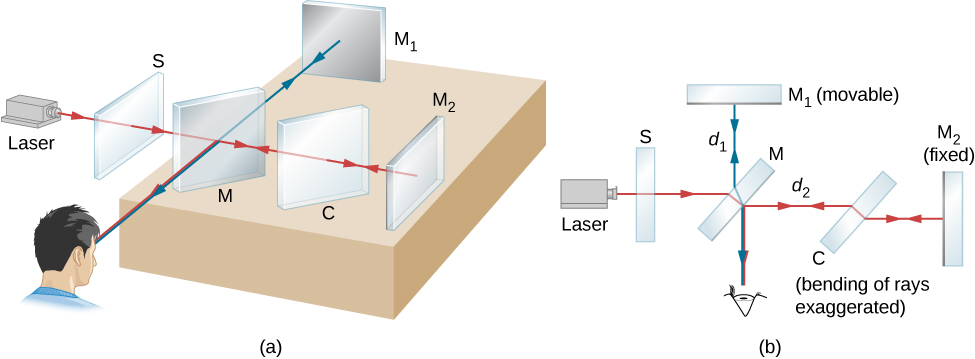
\includegraphics[width=12cm]{src/MichInt.jpg}
    \caption{Michelson干涉仪示意}
\end{figure}
\begin{figure}[ht]
    \centering
    \begin{subfigure}{2cm}
        \centering
        \incfig{2cm}{MichelsonA}
        \caption{}
    \end{subfigure}
    \begin{subfigure}{2cm}
        \centering
        \incfig{2cm}{MichelsonB}
        \caption{}
    \end{subfigure}
    \begin{subfigure}{2cm}
        \centering
        \incfig{2cm}{MichelsonBlack}
        \caption{}
    \end{subfigure}
    \begin{subfigure}{2cm}
        \centering
        \incfig{2cm}{MichelsonB}
        \caption{}
    \end{subfigure}
    \begin{subfigure}{2cm}
        \centering
        \incfig{2cm}{MichelsonA}
        \caption{}
    \end{subfigure}
        \begin{subfigure}{2cm}
        \centering
        \incfig{2cm}{MichelsonBlack}
        \caption{}
    \end{subfigure}
    \begin{subfigure}{2cm}
        \centering
        \incfig{2cm}{MichelsonG}
        \caption{}
    \end{subfigure}
    \begin{subfigure}{2cm}
        \centering
        \incfig{2cm}{MichelsonH}
        \caption{}
    \end{subfigure}
    \begin{subfigure}{2cm}
        \centering
        \incfig{2cm}{MichelsonI}
        \caption{}
    \end{subfigure}
    \begin{subfigure}{2cm}
        \centering
        \incfig{2cm}{MichelsonBlack}
        \caption{}
    \end{subfigure}
    \caption{Michelson干涉仪的各种干涉条纹}
    \label{fig:Michelson干涉仪的各种干涉条纹}
\end{figure}
\begin{figure}[ht]
    \centering
    \begin{subfigure}{2cm}
        \centering
        \incfig{2cm}{MichelsonConfigA}
        \caption{}
    \end{subfigure}
    \begin{subfigure}{2cm}
        \centering
        \incfig{2cm}{MichelsonConfigB}
        \caption{}
    \end{subfigure}
    \begin{subfigure}{2cm}
        \centering
        \incfig{2cm}{MichelsonConfigC}
        \caption{}
    \end{subfigure}
    \begin{subfigure}{2cm}
        \centering
        \incfig{2cm}{MichelsonConfigD}
        \caption{}
    \end{subfigure}
    \begin{subfigure}{2cm}
        \centering
        \incfig{2cm}{MichelsonConfigE}
        \caption{}
    \end{subfigure}
        \begin{subfigure}{2cm}
        \centering
        \incfig{2cm}{MichelsonConfigF}
        \caption{}
    \end{subfigure}
    \begin{subfigure}{2cm}
        \centering
        \incfig{2cm}{MichelsonConfigG}
        \caption{}
    \end{subfigure}
    \begin{subfigure}{2cm}
        \centering
        \incfig{2cm}{MichelsonConfigH}
        \caption{}
    \end{subfigure}
    \begin{subfigure}{2cm}
        \centering
        \incfig{2cm}{MichelsonConfigI}
        \caption{}
    \end{subfigure}
    \begin{subfigure}{2cm}
        \centering
        \incfig{2cm}{MichelsonConfigJ}
        \caption{}
    \end{subfigure}
    \caption{\cref{fig:Michelson干涉仪的各种干涉条纹}中对应条纹的仪器位置}
    \label{fig:对应条纹的仪器位置}
\end{figure}
如\cref{fig:Michelson干涉仪的各种干涉条纹}中的条纹和\cref{fig:对应条纹的仪器位置}中的相应仪器位置. $M_2'\parallelsum M_1$时发生等倾干涉. 点光源入射, 较远密而弱, 中心斑点小. 较近疏而强, 中心斑点大, 重合时中心斑点扩大到整个视场. 镜面相互靠近则条纹不断锁进中心, 反之条纹不断由中心生出.
\par
若$M_2'$和$M_1$之间有夹角, 则以扩展光源入射时, 较远几乎看不到条纹, 较近有弯曲的条纹, 相交时会有直条纹. 镜面相互靠近, 朝曲率小的方向移动, 反衬度不断变大. 镜面相互远离, 朝曲率大的方向移动, 反衬度不断降低.
\par
条纹会向高$h$处弯曲. 在$M_1$和$M_2$的交点处条纹为直线.
\par
\begin{remark}
    激光/近平行光入射, 不相交位置也是平行条纹.
\end{remark}
\begin{remark}
    两镜子的夹角趋于零, 则一个竖条纹逐渐被拉宽, 扩展至整个视场.
\end{remark}
\par
白光照明时, $0$级条纹不发生色散, 可以由此找到等光程点.

\paragraph{双色光入射} % (fold)
\label{par:双色光入射}

例如钠光灯波长为$\SI{589.0}{\nano\meter}$和$\SI{589.6}{\nano\meter}$.
\begin{align*}
    &\begin{cases}
        I_1 \pare{\Delta L} = I_0\brac{1+\cos\pare{k_1\Delta L}}, \\
        I_2 \pare{\Delta L} = I_0\brac{1+\cos\pare{k_2\Delta L}}.
    \end{cases}\\
    I\pare{\Delta L} &= I_1 + I_2 = 2I_0 \brac{1 + \cos\pare{\frac{\Delta k\Delta L}{2}}\cos\pare{k\Delta L}}.
\end{align*}
其中$\Delta k = k_1 + k_2,\displaystyle k = \frac{k_1+k_2}{2}$. 故$\displaystyle \gamma = \abs{\cos \frac{\Delta k \Delta L}{2}}$. 可见度会发生振荡, 其周期为
\begin{align*}
    \Delta L &= \frac{2\pi}{\Delta k} = \frac{2\pi}{k_1 - k_2} \\
    &= \frac{\lambda_1 \lambda_2}{\lambda_2 - \lambda_1} \sim \frac{\lambda^2}{\Delta\lambda}.
\end{align*}
对应的条纹数$\displaystyle N = \frac{\Delta L}{\lambda} = \frac{\lambda}{\Delta\lambda}$. 空间频率为$\displaystyle f = \rec{\Delta L} = \Delta \lambda / \lambda^2$.

% paragraph 双色光入射 (end)

\paragraph{展宽光源} % (fold)
\label{par:展宽光源}

设光强在$k$空间内均匀分布, 展宽$k_0 \pm \Delta k / 2$, 则
\begin{align*}
    I &= I_0 \pare{1 + \rec{\Delta k} \int_{k-\Delta k/2}^{k+\Delta k/2} \cos \pare{k\Delta L}\,\rd{k}}\\
    I &= I_0 \brac{1 + \frac{\sin \frac{\Delta k \Delta L}{2}}{\frac{\Delta k \Delta L}{2}}\cos\pare{k\Delta L}},\\
    \gamma &= \abs{\sinc \frac{\Delta k\Delta L}{2}}.
\end{align*}
最大光程差$\displaystyle \delta L_m = \frac{2\pi}{\Delta k} = \frac{\lambda^2}{\Delta \lambda}$.

% paragraph 展宽光源 (end)

\paragraph{光场的时间相干性} % (fold)
\label{par:光场的时间相干性}

单色平面波$\displaystyle \tilde{U}\pare{x} = \tilde{A} e^{-ikx}$在时间上无穷, 而具有展宽的波列
\begin{align*}
    \tilde{U}\pare{x} &= \frac{\tilde{A}}{\Delta k} \int_{k-\Delta k/2}^{k+\Delta k/2} e^{-ikx}\,\rd{x} \\
    &= \tilde{A} \sinc \pare{\frac{\Delta k}{2}x}e^{-ikx}. 
\end{align*}
当$\abs{x} = \lambda^2/\Delta\lambda$, 振幅为零. 定义波列长$L_0 = \lambda^2/\Delta \lambda$. 注意这和之前的$\Delta l_m$相同. 相应的传播时间为$\tau_0 = L_0/c \sim 1/\Delta \nu$, 即$\tau_0 \Delta \nu \sim 1$, 这是\emph{时间相干性的反比公式}.

% paragraph 光场的时间相干性 (end)

\begin{sample}
    \begin{ex}
        连续单频激光器($\SI{1}{\kilo\hertz}$线宽), 经过斩波器获得$\SI{10}{\nano\second}$宽的脉冲, 再经过$\SI{1}{\kilo\hertz}$的频谱滤波器.
        \begin{cenum}
            \item 连续激光脉冲通过滤波器的透过率为$100$\%;
            \item 脉冲透过率为$\eta = \displaystyle \frac{\SI{1}{\kilo\hertz}}{\SI{100}{\mega\hertz}} = 10^{-5}$;
            \item 透过后的时间宽度为$\SI{1}{\milli\second}$.
            \item 如果最后一个滤波器的线宽是$\SI{10}{\nano\second}$, 则透过率为$100\%$, 而透过后的时间宽度为$\SI{10}{\nano\second}$.
        \end{cenum}
    \end{ex}
\end{sample}
\begin{sample}
    \begin{ex}
        连续单频激光器$\SI{1}{\kilo\hertz}$线宽, 经过斩波. 计划测量一个$\SI{1}{\mega\hertz}$线宽的原子吸收线, 测量光谱的宽度至少为$\SI{1}{\micro\second}$.
    \end{ex}
\end{sample}
\begin{sample}
    \begin{ex}
        连续单频激光器($\SI{1}{\kilo\hertz}$线宽)经过高速声光晶体实现频率扫描. 现在目标扫描范围$\SI{5}{\mega\hertz}$, 目标扫描精度需要达到$\SI{10}{\kilo\hertz}$. 试设计扫频的时长及离散点数.
    \end{ex}
    \begin{proof}[解]
        点数$\displaystyle \frac{5\times 10^6}{10\times 10^3} = 500$. $\Delta \nu < \SI{10}{\kilo\hertz}$, 故$\Delta t > \SI{100}{\micro\second}$.
    \end{proof}
\end{sample}

\paragraph{作业} % (fold)
\label{par:作业}

p.300 2, 3, 5, 6 (p.200)

% paragraph 作业 (end)

\par
时间相干性的表达式为$\tau_0 \cdot \Delta \nu = 1$, 空间相干性为$b\cdot \Delta \theta = \lambda$. 前者主要体现在分振幅干涉, 后者主要体现在分波前干涉.
\par
空间相干性来源于扩展光源不同部分的发光独立性; 时间相干性来源于光源发光过程在时间上的断续性. 从后果上看, 空间相干性主要表现在波前, 时间相干性主要表现在波列.
\par
实际光源的扩展性引入空间相干性. 非单色性引入时间相干性.

\begin{sample}
    \begin{ex}
        在Michelson干涉仪中, 若假设光速并非不变, 则将干涉仪旋转$\SI{90}{\degree}$会导致光程变化, 从而条纹将移动. 推算得条纹$\Delta N = 0.4$, 但实际中并未观察到.
    \end{ex}
\end{sample}

\subsubsection{Fourier变换光谱仪} % (fold)
\label{ssub:fourier变换光谱仪}

从干涉的结果得到光谱的分布,
\[ I\pare{\Delta L} - I_0 = \rec{\pi} \int_0^\infty i\pare{k}\cos\pare{k\Delta L}\,\rd{k}. \]
逆变换
\[ i\pare{k} = 2\int_0^\infty \brac{I\pare{\Delta L} - I_0}\cos\pare{k\Delta L}\,\rd{\pare{\Delta L}}. \]
在Michelson干涉仪中令$M_2$以速度$v$外移而, 从而$\Delta L = vt$. 记录每一时刻的$t$, 从而得到$I\pare{\Delta L}$, 逆变换可得$i\pare{k}$.

\paragraph{作业} % (fold)
\label{par:作业}

p.329-330 2, 3, 4, 6, 7 (p.241) 与思考题: Michelson干涉仪还有哪些可能的应用

% paragraph 作业 (end)

% subsubsection fourier变换光谱仪 (end)

% subsection michelson干涉仪 (end)

\subsection{Fabry-P\texorpdfstring{\'e}{e}rot干涉仪} % (fold)
\label{sub:fabry_perot干涉仪}

\begin{figure}[ht]
    \centering
    \incfig{11cm}{MultiInterference}
    \caption{多光束干涉}
    \label{fig:多光束干涉}
\end{figure}
在如\cref{fig:多光束干涉}的多光束干涉中, 光程差和相位差
\[ \Delta l = 2nh\cos i, \quad \delta = \frac{4\pi}{\lambda}nh\cos i. \]
假设$n_1 = n_2$, 则$r' = -r$, $rr'+tt' = 1$. 反射
\[ A1 = Ar,\quad A_2 = Atr't' = -Atrt',\quad A_3 = Atr'^3 t' = -Atr^3 t',\quad \cdots. \]
透射
\[ A'_1 = Att',\quad A'_2 = Atr'r't' = Atr^2 t',\quad A'_3 = Atr^4 r',\quad \cdots. \]
简化$r\ll 1$且$t,t'\sim 1$, 则
\[ \tilde{U}_T = Att' e^{i\delta/2} \pare{1+r^2 e^{i\delta} + r^4 e^{i2\delta} + \cdots} = \frac{Att'}{1-r^2 e^{i\delta}}. \]
从而透射强度
\[ I_T = \tilde{U}_T^* \tilde{U}_T = \frac{A^2\pare{tt'}^2}{\pare{1-r^2e^{i\delta}}\pare{1-r^2e^{-i\delta}}}. \]
其中$tt' = 1-r^2$, $A^2 = I_0$, $I_T = \displaystyle\frac{I_0\pare{1-r^2}^2}{1+r^4-2r^2\cos\delta}$. 而$R=r^2$, 故
\[ I_T = \frac{I_0}{1+\frac{4R\sin^2\pare{\delta/2}}{\pare{1-R}^2}},\quad I_R = I_0 - I_T = \frac{I_0}{1+\frac{\pare{1-R}^2}{4R\sin^2\pare{\delta/2}}}. \]
光强$I_R$和$I_T$仅于$\delta$有关, 而$\delta$与$h$, $i$有关.
\[ \begin{cases}
    \delta = 2k\pi,& I_T = I_0,\quad I_R = 0; \\
    \delta = \pare{2k+1}\pi,& I_T = 0,\quad I_R = I_0.
\end{cases} \]
当$R\ll 1$, 有
\[ \begin{cases}
    I_T &= I_0\pare{1-2R\pare{1-\cos\delta}} \approx I_0,\\
    I_R &= 2RI_0\pare{1-\cos\delta}.
\end{cases} \]
当$R$变大, 透射条纹将变细. 在$I_T$极大值处, $\delta = 2k\pi$而$\sin\delta\rightarrow 0$. 由于$\displaystyle\frac{4R}{\pare{1-R}^2}$随$R$递增, 故$\delta$的条件更难满足, 故条纹变细.
\begin{figure}[ht]
    \centering
    \incfig{8cm}{FabryPeroInterferometerBasic}
\end{figure}
\par
F-P腔可作为干涉滤波片. 可以通过Air Space或固体材料两面镀高反膜实现.
\par
当$\delta = 2k\pi$, $I_T/I_0 = 0$, $\displaystyle \delta = \frac{4\pi nh\cos i}{\lambda_k} = 2k\pi\Rightarrow$正入射时
\[ \lambda_k = \frac{2nh}{k},\quad \nu_k = \frac{kc}{2nh}. \]
故模式间距$\Delta \nu = \nu_{k+1} - \nu_k = \displaystyle \frac{c}{2nh}$.
\par
设半峰宽度$\epsilon$使得$I\pare{\delta = 2k\pi \pm \epsilon/2} = I_0/2$, 则
\[ \half = \rec{1+\frac{4R\sin^2\frac{\delta}{2}}{1-R}} \sim \rec{1+\frac{R\epsilon^2}{4\pare{1-R}^2}}. \]
故$\epsilon = \displaystyle \frac{2\pare{1-R}}{\sqrt{R}}. $当$R\rightarrow\infty$, 有$\epsilon\rightarrow 0$.
\par
固定$\lambda$, 令$i$变化, 考虑到$\displaystyle \delta = \frac{4\pi nh\cos i}{\lambda_k}$,
\[ \+did\delta = -\frac{4\pi nh\sin i}{\lambda}, \]
从而当$\delta$跨过$\epsilon$,
\[ \Delta i_k = \frac{\lambda\epsilon}{2\pi nh\sin i_k} = \frac{\lambda}{4\pi nh\sin i_k}\cdot \frac{2\pare{1-R}}{\sqrt{R}}. \]
从而$R$增加, 或$h$增加, 或$i$增加都会导致条纹更细锐.
\par
若固定正入射$i=0$, $\lambda$变化, 则$\rd{\delta}$跨过$\epsilon$时,
\[ \+d\lambda d\delta = -\frac{4\pi nh\cos i}{\lambda^2} \Rightarrow \Delta\lambda_k = \frac{\lambda^2\epsilon}{4\pi nh\cos i}. \]
\[ \frac{\Delta \nu}{\nu_0} = \frac{\Delta\lambda}{\lambda_0} \Rightarrow \Delta\nu_k = c\frac{\Delta \lambda_k}{\lambda_k} = \frac{c}{\pi k\lambda} \cdot \frac{1-R}{\sqrt{R}}. \]
故当$R$上升, $\Delta \nu_k$和$\Delta \lambda_k$下降, 谱分辨率上升.
\begin{remark}
    Rayleigh判据谓两谱线中心角距离等于半值角宽度时可分辨.
\end{remark}
分辨质量
\[ Q = \frac{\lambda}{\Delta \lambda} = \frac{\pi k\sqrt{R}}{1-R}. \]
当$R$上升时, $Q$会上升. 定义精细度(Finesse)
\[ F = \frac{\pi \sqrt{R}}{1-R} \Rightarrow Q = kF. \]
其中$k$为干涉级次$\displaystyle k=\frac{2nh}{\lambda}$.
\par
FSR$= \displaystyle \frac{c}{2nh}$当$h$下降时会上升.
\begin{remark}
    实际中通常先粗滤波至$\SI{1}{\nano\meter}$范围, 后通过FB干涉仪将精度调节至$\SI{e-3}{\nano\meter}$.
\end{remark}

\subsubsection{多层膜的反射和透射} % (fold)
\label{ssub:多层膜的反射和透射}

\begin{figure}[ht]
    \centering
    \incfig{4cm}{MultipleTransRefl}
\end{figure}
假设$m$层和$m-1$层的反射和透射率为$r_m,t_m$和$r_{m-1}$, $t_{m-1}$, 类似于前面多光束干涉的推导得到诸层的$R$和$T$.

% subsubsection 多层膜的反射和透射 (end)

% subsection fabry_perot干涉仪 (end)

% section 光的干涉 (end)

\end{document}
